
\section{ソフトウェア}
  \subsection{自己位置推定}
  ロボカーの中心が点$(x_k,y_k)$の位置にあるとし、時間$\Delta t$秒の間にロボカーが旋回中心の周りに$\Delta \theta$だけ回転したとする.このときロボカーの中心から車輪までの距離を$d$,左右の車輪とロボカーの中心が動いた距離をそれぞれ$\Delta L_R, \Delta L_L, \Delta L$とすると
\begin{equation}
   \Delta L_R = (\rho + d) \Delta \theta \nonumber
\end{equation}
\begin{equation}
  \Delta L_L  =  (\rho - d) \Delta \theta \nonumber
\end{equation}
\begin{equation}
   \Delta L  = \rho \Delta \theta
\end{equation}
 

  となる.これより
  \begin{eqnarray}
   \Delta L &=& \frac{\Delta L_R + \Delta L_L}{2} \nonumber \\
   \Delta \theta &=& \frac{\Delta L_R - \Delta L_L}{2}
    \label{eq:eq1}
  \end{eqnarray}
  が得られる.\\
  図\ref{fig:fig1}より,オドメトリを用いた自己位置推定による位置の更新式は次のようになる.
   \begin{eqnarray}
    \left[
     \begin{array}{c}
      x_{k+1} \\
      y_{k+1} \\ 
      \theta_{k+1} \\
     \end{array}d
	\right]
    = \left[
       \begin{array}{c}
 x_k \\ 
 y_k \\
 \theta_k \\
       \end{array}
\right]
+ \left[
\begin{array}{c}
 \Delta L \cos(\theta_k + \frac{\Delta \theta}{2}) \\
 \Delta L \sin(\theta_k + \frac{\Delta \theta}{2}) \\
 \Delta \theta\\
\end{array}
\right]
   \end{eqnarray}
ここで,式\ref{eq:eq1}より
\begin{equation}
\left[
 \begin{array}{c}
  x_{k+1} \\
  y_{k+1} \\
  z_{k+1} \\
 \end{array}
\right] 
= \left[
\begin{array}{c}
 x_k \\
 y_k \\
 z_k \\
\end{array}
\right]
+ \left[
\begin{array}{cc}
 \frac{\cos(\theta_k) + \frac{\Delta \theta}{2}}{2} & \frac{\cos(\theta_k) + \frac{\Delta \theta}{2}}{2} \\
 \frac{\sin(\theta_k) + \frac{\Delta \theta}{2}}{2} & \frac{\sin(\theta_k) + \frac{\Delta \theta}{2}}{2} \vspace{1mm}\\
 \frac{1}{2d} & -\frac{1}{2d} \\
\end{array}
\right]
\left[
\begin{array}{c}
 \Delta L_R \\
 \Delta L_L \\
\end{array}
\right]
\end{equation}
となる.

\begin{figure}[H]
 \begin{center}
  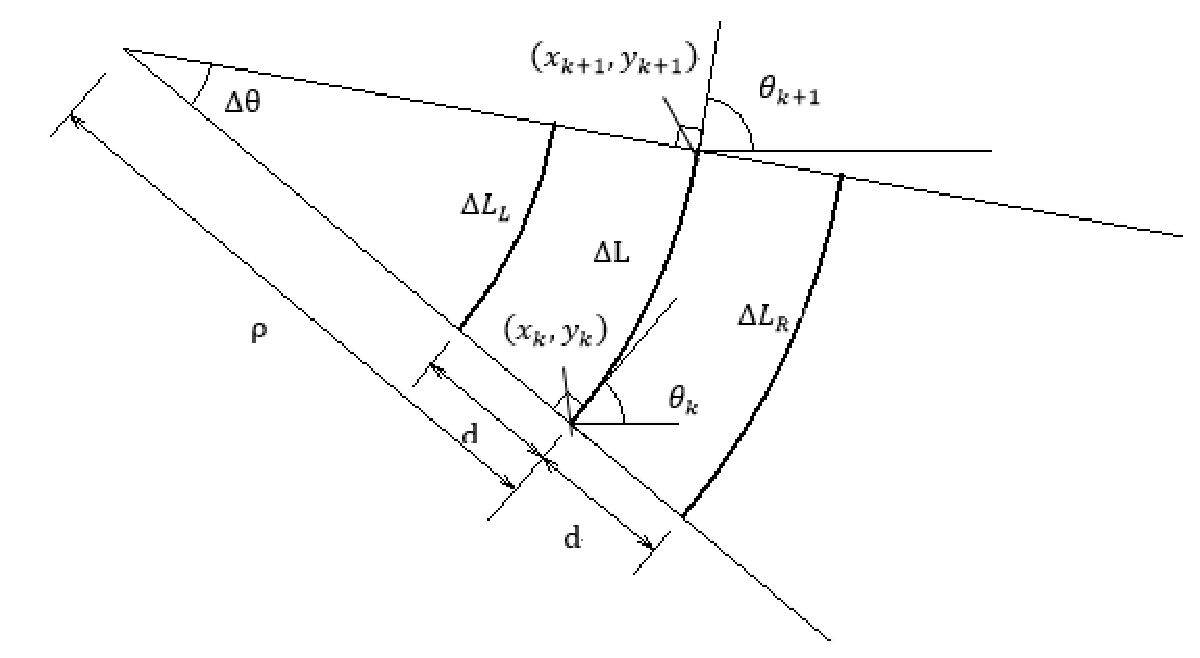
\includegraphics[scale = 0.5]{../odom/picture/odom.eps}
  \caption{自己位置推定}
  \label{fig:fig1}
 \end{center}
\end{figure}
